\documentclass[10pt]{beamer}
\usepackage[utf8]{inputenc}
\usepackage{graphicx}
\usepackage[export]{adjustbox}
\usepackage {mathtools}
\usepackage{listings}
\definecolor{mygreen}{rgb}{0,0.6,0}
\definecolor{mygray}{rgb}{0.5,0.5,0.5}
\definecolor{mymauve}{rgb}{0.58,0,0.82}
\lstset{
  %basicstyle=\fontsize{8}{10}\selectfont\ttfamily,%\footnotesize,        % the size of the fonts that are used for the code
  basicstyle=\ttfamily,
  breakatwhitespace=false,         % sets if automatic breaks should only happen at whitespace
  breaklines=false,                % sets automatic line breaking
  captionpos=b,                    % sets the caption-position to bottom
  columns=fixed,
  commentstyle=\color{mygreen},    % comment style
  extendedchars=true,              % lets you use non-ASCII characters; for 8-bits encodings only, does not work with UTF-8
  keepspaces=true,                 % keeps spaces in text, useful for keeping indentation of code (possibly needs columns=flexible)
  keywordstyle=\color{blue},       % keyword style
  %language=[95]Fortran,            % the language of the code
  numbers=none,                    % where to put the line-numbers; possible values are (none, left, right)
  numbersep=5pt,                   % how far the line-numbers are from the code
  numberstyle=\tiny\color{mygray}, % the style that is used for the line-numbers
  rulecolor=\color{black},         % if not set, the frame-color may be changed on line-breaks within not-black text (e.g. comments (green here))
  showspaces=false,                % show spaces everywhere adding particular underscores; it overrides 'showstringspaces'
  showstringspaces=false,          % underline spaces within strings only
  showtabs=false,                  % show tabs within strings adding particular underscores
  stepnumber=1,                    % the step between two line-numbers. If it's 1, each line will be numbered
  %stringstyle=\color{mymauve},     % string literal style
  tabsize=4,                       % sets default tabsize to 2 spaces
  %title=\lstname                   % show the filename of files
}
\usepackage{utopia} %font utopia imported
\usetheme{CambridgeUS}
\usecolortheme{dolphin}

% set colors
\definecolor{myNewColorA}{RGB}{153,208,109}
\definecolor{myNewColorB}{RGB}{109,188,47}
\definecolor{myNewColorC}{RGB}{76,132,33}
\setbeamercolor*{palette primary}{bg=myNewColorC}
\setbeamercolor*{palette secondary}{bg=myNewColorB}
\setbeamercolor*{palette tertiary}{bg=myNewColorA}
\setbeamercolor*{titlelike}{fg=myNewColorB}
\setbeamercolor*{title}{bg=myNewColorA}
\setbeamercolor*{item}{fg=myNewColorA}
\setbeamercolor*{caption name}{fg=myNewColorA}
\setbeamercolor{frametitle}{fg=myNewColorC}

\usepackage{braket}
\usepackage{amssymb}
\usepackage{dutchcal}
\usepackage{ifsym}
\usepackage[T1]{fontenc} % if needed
\usepackage{bm}
\usepackage{bbm}
\usepackage{slashed}
\usepackage{dashrule}
\usepackage{pifont}

\newcommand{\ds}[1]{\slashed{#1}}

\usepackage{graphicx}%

\usepackage{tikz}
\newcommand*\circled[1]{\tikz[baseline=(char.base)]{
            \node[shape=circle,draw,inner sep=2pt] (char) {#1};}}
\usetikzlibrary{decorations.pathmorphing}
\usetikzlibrary{decorations.markings}
\usetikzlibrary{patterns}
\usetikzlibrary{calc}
\usetikzlibrary{math}
\usetikzlibrary{fpu}
\usepackage{standalone}
\usepackage{pgffor}
\usepackage{booktabs} % for '\midrule' macro
\usepackage{amsmath}  % for '\overset' macro
%\usepackage{newpxmath,newpxtext}

\usepackage{hhline}

\usepackage{parskip}

% Mathematica code
\usepackage{lmodern}
\usepackage{mmacells}
% --------------------------------------------------
% Color packages and definitions
\usepackage[most]{tcolorbox}
\usepackage{xcolor}
\definecolor{myGreen}{rgb}{0.2,0.72,0.2}
\definecolor{greengray}{rgb}{0.7,0.8,0.7}
\definecolor{bluegray}{rgb}{0.7,0.7,0.85}
\definecolor{redgray}{rgb}{0.85,0.7,0.7}
\definecolor{myWhite}{rgb}{0.98,0.98,0.98}
\definecolor{myGray}{rgb}{0.7,0.7,0.75}
\definecolor{myGold}{rgb}{0.8,0.64,0.24}
\definecolor{myYellow}{rgb}{1.0,1.0,0.69}
\newcommand{\new}[1]{{\sf\color{red}{#1}}}
\newcommand{\green}[1]{\textcolor{myGreen}{#1}}
\newcommand{\red}[1]{\textcolor{red}{#1}}
\newcommand{\blue}[1]{\textcolor{blue}{#1}}
\newcommand{\white}[1]{\textcolor{myWhite}{#1}}
\newcommand{\gold}[1]{\textcolor{myGold}{#1}}
% \renewcommand{\section}[1]{\newpage\section{{#1}}}
% --------------------------------------------------

% --------------------------------------------------
% Custom comands
\DeclareMathOperator*{\SumInt}{%
\mathchoice%
  {\ooalign{$\displaystyle\sum$\cr\hidewidth$\displaystyle\int$\hidewidth\cr}}
  {\ooalign{\raisebox{.14\height}{\scalebox{.7}{$\textstyle\sum$}}\cr\hidewidth$\textstyle\int$\hidewidth\cr}}
  {\ooalign{\raisebox{.2\height}{\scalebox{.6}{$\scriptstyle\sum$}}\cr$\scriptstyle\int$\cr}}
  {\ooalign{\raisebox{.2\height}{\scalebox{.6}{$\scriptstyle\sum$}}\cr$\scriptstyle\int$\cr}}
}

\newcommand\myfontsize{\fontsize{8pt}{9.6pt}\selectfont}
\newcommand\smallfonteq{\fontsize{9pt}{10.8pt}\selectfont}

\newcommand{\highlight}[1]{\colorbox{myYellow}{\text{${#1}$}}}

\newcommand{\ok}{\green{\ding{51}}}
\newcommand{\wrong}{\red{\ding{55}}}
\newcommand{\semidone}{\ding{122}}
\newcommand{\todo}{$\square$}

\newcommand{\sign}{\text{sign}}


\newcommand{\et}{\varepsilon_{T}}
\newcommand{\vetp}[1]{\bm{#1}_{T}}
\newcommand{\xup}{x_{123},\vetp{b}}
\newcommand{\xdo}{x_{321},\vetp{b}}
\newcommand{\e}{\varepsilon}
\newcommand{\ta}{\left(}
\newcommand{\qa}{\left[}
\newcommand{\ga}{\left\{}
\newcommand{\tc}{\right)}
\newcommand{\qc}{\right]}
\newcommand{\gc}{\right\}}
\newcommand{\tr}[1]{\text{Tr}\qa {#1} \qc}
\renewcommand{\[}{\begin{equation*}}
\renewcommand{\]}{\end{equation*}}
\newcommand{\nb}{{\bar{n}}}

% Mathematica code stuff

\mmaDefineMathReplacement[≤]{<=}{\leq}
\mmaDefineMathReplacement[≥]{>=}{\geq}
\mmaDefineMathReplacement[≠]{!=}{\neq}
\mmaDefineMathReplacement[→]{->}{\to}[2]
\mmaDefineMathReplacement[⧴]{:>}{:\hspace{-.2em}\to}[2]
\mmaDefineMathReplacement{∉}{\notin}
\mmaDefineMathReplacement{∞}{\infty}
\mmaDefineMathReplacement{��}{\mathbbm{d}}

\mmaSet{
  morefv={gobble=2},
  linklocaluri=mma/symbol/definition:#1,
  morecellgraphics={yoffset=1.9ex}
}

% new \oset macro:
\makeatletter
\newcommand{\oset}[3][0ex]{%
  \mathrel{\mathop{#3}\limits^{
    \vbox to#1{\kern-2\ex@
    \hbox{$\scriptstyle#2$}\vss}}}}
\makeatother

\renewcommand{\l}{\lambda}
\newcommand{\m}{\mu}
\newcommand{\lb}{{\bar{\lambda}}}
\newcommand{\mb}{{\bar{\mu}}}

\newcommand{\f}{f_{++}}
\newcommand{\fb}{\bar{f}_{++}}
\newcommand{\p}{\psi_\lambda}
\newcommand{\ps}{\bar{\psi}_{\bar{\lambda}}}

\newcommand{\rDer}[1]{\oset[-0.2ex]{\rightarrow}{#1}\phantom{\,}}
\newcommand{\lDer}[1]{\oset[-0.2ex]{\leftarrow}{#1}\phantom{\,}}
\newcommand{\lrDer}[1]{\oset[-0.2ex]{\leftrightarrow}{#1}\phantom{\,}}

\newcommand{\whiteline}{\vskip 0.5cm}
%\newcommand{\myline}[1]{{\color{#1}\rule{\textwidth}{2pt}}\\}
\newcommand{\myline}[1]{{\color{#1}\center\hdashrule[1.0ex]{1\linewidth}{2pt}{1.5mm}}\\}
\newcommand{\mydoubleline}[1]{{\color{#1}\center\hdashrule[-8.5ex]{1\linewidth}{2pt}{1.5mm}}
{\color{#1}\center\hdashrule[0.0ex]{1\linewidth}{2pt}{1.5mm}}\\}

\usefonttheme{professionalfonts}
\usepackage{natbib}
\usepackage{hyperref}
\hypersetup{colorlinks,
citecolor=myNewColorC,
linkcolor=.,
menucolor=white,
filecolor=pink,   
anchorcolor=yellow
    }
%------------------------------------------------------------
% \titlegraphic{\includegraphics[height=2cm]{hku-logo-eps.eps}}

\setbeamerfont{title}{size=\large}
\setbeamerfont{subtitle}{size=\small}
\setbeamerfont{author}{size=\small}
\setbeamerfont{date}{size=\small}
\setbeamerfont{institute}{size=\small}
\title{Neural Networks for physics}
\author[S. Rodini]{Simone Rodini}


\date[\today]{\today}

%\date[Hong Kong 2024.1]
%{Hong Kong 2024.1}


%------------------------------------------------------------
%This block of commands puts the table of contents at the 
%beginning of each section and highlights the current section:
\AtBeginSection[]
{
 \begin{frame}
   \frametitle{Contents}
   \tableofcontents[currentsection]
 \end{frame}
}
\AtBeginSection[]{
  \begin{frame}
  \vfill
  \centering
  \begin{beamercolorbox}[sep=8pt,center,shadow=true,rounded=true]{title}
    \usebeamerfont{title}\insertsectionhead\par%
  \end{beamercolorbox}
  \vfill
  \end{frame}
}
%------------------------------------------------------------

\begin{document}

%The next statement creates the title page.
\frame{\titlepage}
\begin{frame}
\frametitle{Contents}
\tableofcontents
\end{frame}
%------------------------------------------------------------
\section{}
\begin{frame}{Outline}
How does a computer think? 
\begin{enumerate}
\item How does a digital computer actually think? A brief window on machine instructions, assembly and programming languages.
\item How can we make a higher-level model of intelligence (or logical reasoning) on a machine? Neural Networks demystified.
\item A specific application: how to use a NN to model an unknown physics phenomena.
\end{enumerate}
\end{frame}

\section{Computer basics}
\subsection{Numbers on a computer}

\begin{frame}{A general idea}
\begin{columns}
\begin{column}{0.3\textwidth}
\newline
\begin{figure}
\centering
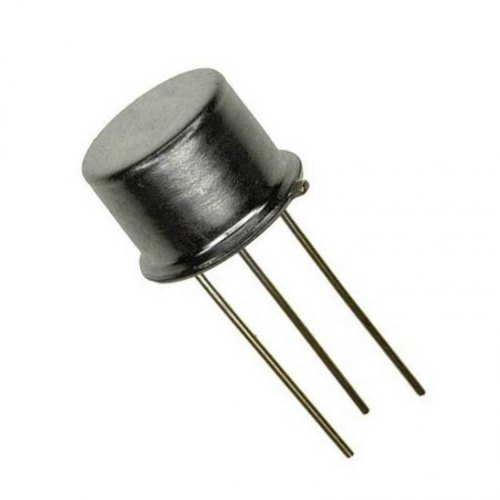
\includegraphics[width=0.25\textwidth]{Notes/Figures/transistor.jpg}
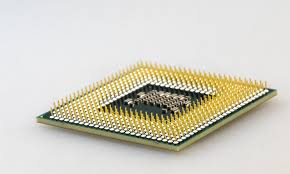
\includegraphics[width=0.45\textwidth]{Notes/Figures/cpu.jpeg}

\end{figure}
\end{column}

\begin{column}{0.7\textwidth}
Transistors: the foundation
\end{column}
\end{columns}
\pause
\begin{figure}
\centering
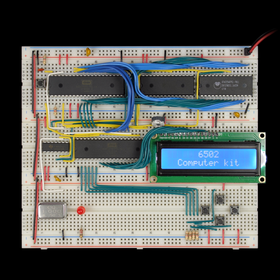
\includegraphics[width=0.35\textwidth]{Notes/Figures/6502_280x420.png}
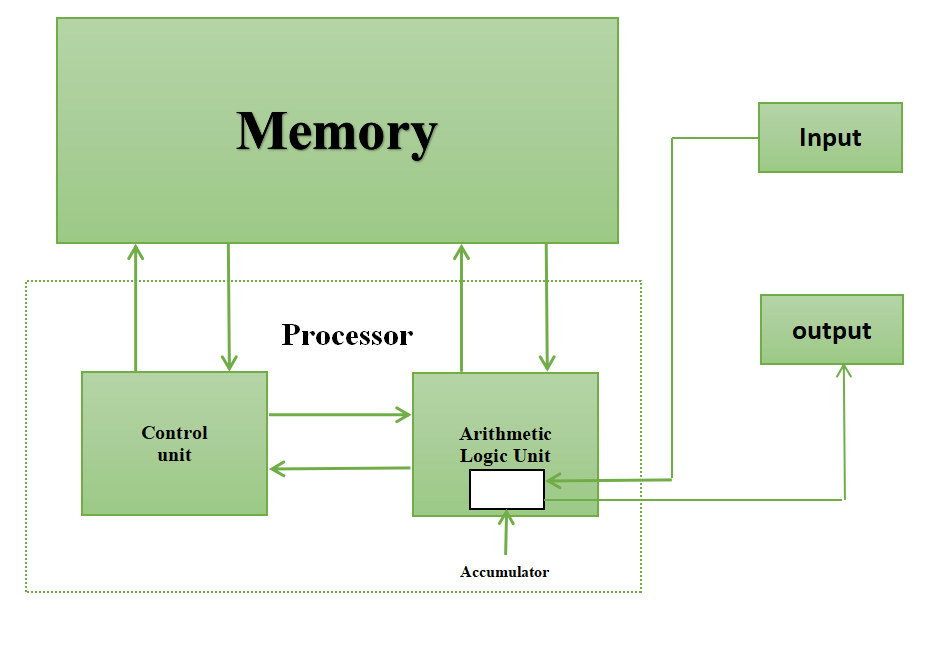
\includegraphics[width=0.6\textwidth]{Notes/Figures/cpu_diagram.png}
\end{figure}
\end{frame}

\begin{frame}{Number representation}
\begin{columns}
\begin{column}{0.5\textwidth}
All digital computer works storing information as voltage level.\\
We can store \red{2} values, conventionally referred to as \red{0, 1}.
\end{column}

\begin{column}{0.5\textwidth}
\begin{figure}
\centering
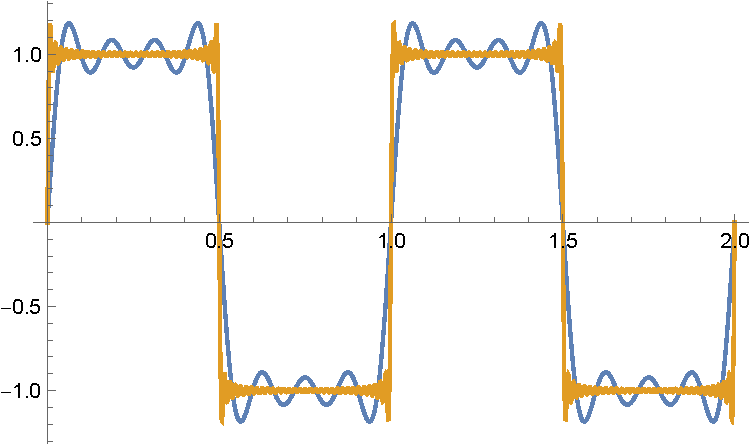
\includegraphics[width=\textwidth]{Notes/Figures/square_wave.pdf}
\end{figure}
\end{column}
\end{columns}
\pause
\red{Why not more?} Possible, but it has costs: energy, reliability, scalability etc... \\
How can we represent numbers using only $0,1$? Binary!\\
How to read a \red{base-10} number?
\[
\underset{\quad \quad \quad \hookleftarrow}{6710597111_{\red{10}}} \equiv 1 \cdot 10^0 +  1 \cdot 10^1 + 1 \cdot 10^2 + 7 \cdot 10^3 +...
\]
So, binary = base-2:
\[
11011011_{\red{2}} = 1 \cdot 2^0 + 1 \cdot 2^1 + 0 \cdot 2^2 + 1 \cdot 2^3 +  ...
\]

\end{frame}

\begin{frame}{Number representation}
Nowadays hardware can manage \red{64 bit} numbers: up to $2^{63}\lesssim 10^{19}$.\\
Inconvenient to think in binary $\Rightarrow$ hexadecimal! Use $0$ and other $15$ symbols to represent numbers: $0,1,...,9,$A,B,C,D,E,F: 
$
\underbrace{1101}_{\text{D}}\underbrace{1011}_{\text{B}} = \text{DB}_{16}
$
% With actually 64 bits:
% \[\begin{split}
% &\underbrace{1101}_{\text{D}}\underbrace{0101}_{\text{5}}\underbrace{0110}_{\text{B}}\underbrace{1111}_{\text{7}}\underbrace{0111}_{\text{C}}\underbrace{0001}_{\text{5}}\underbrace{0110}_{\text{B}}\underbrace{1111}_{\text{7}}\underbrace{0111}_{\text{7}}\underbrace{0111}_{\text{B}}\underbrace{0110}_{\text{7}}\underbrace{1111}_{\text{D}}\underbrace{1100}_{\text{3}}\underbrace{1101}_{\text{A}}\underbrace{0111}_{\text{7}}\underbrace{1011}_{\text{B}} \\ &= \text{D5B7C5B77B7D3A7B}
% \end{split}
% \]

1 bit: one $1$ or $0$, 1 byte: eight $1$ and $0$ like $01000010$ $\equiv$ two hex number $42$.\\
$64$ bits $\equiv$ $8$ bytes.\\
Addition table: \begin{tabular}{c|c|c}
  & 0 & 1 \\
  \hline
0 & 0 & 1\\
1 & 1 & 0$^*$
\end{tabular}  and multiplication table: \begin{tabular}{c|c|c}
  & 0 & 1 \\
  \hline
0 & 0 & 0\\
1 & 0 & 1
\end{tabular}\\
*: carrying the $1$, like in $9+1 = 0$ plus the carried $1$.

\end{frame}

\begin{frame}{Beyond positive integers}
From any base $n$ to decimal is simple. From base-10 to any base: quotient-remainder algorithm: a tiny bit more annoying to carry out.\\
Positive integers \ok\\
Negative integers? Use the most significant bit (the leftmost one) to encode the sign: $0\Rightarrow$ positive. In formulas
\[
b_{N-1}b_{N-2}...b_{0} = -b_{N-1}2^{N-1} + \sum_{i=0}^{N-2}b_{i}2^{i}
\]
\pause
For example:
\[
1001_{2} = -1\cdot 2^3 + 1\cdot 2^0 = -8+1 = -7
\]
Check: $7_{10}$ = $0111_{2}$ and
\begin{columns}
\begin{column}{0.75\textwidth}
\[
\begin{split}
&0^\text{\tiny 1 }1^\text{\tiny 1 }1^\text{\tiny 1 }1 +\\
&1\ \: 0\  0\ \:  1 = \\
\hline 
\red{1}&0\ \: 0\ 0\ \: 0
\end{split}
\] 
\end{column}
\begin{column}{0.25\textwidth}
\begin{figure}
    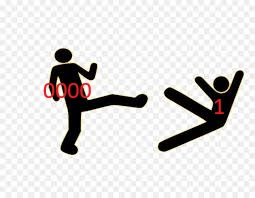
\includegraphics[width=1\textwidth,left]{Notes/Figures/download.jpeg}
    \hfill
\end{figure}

\end{column}
\end{columns}
\end{frame}

\begin{frame}{Floating Point}
How to represent numbers that are not integers?\\
In binary we can use inverse powers of $2$, for instance $0.1_2 \equiv 1\cdot 2^{-1}$. \\
A curiosity: whether a number as a periodical form \red{depends} on the base! For instance $1/5 = 0.2_{10}$ in binary is $0.001\ 1001\ 1001\ ..._{2}$.

On a computer only so many bits: no real numbers!\\
Could we reserve some bits for the part after the period? Like
\[
\underbrace{101...1}_{\text{32-bit}}\red{.}\underbrace{110...1}_{\text{32-bit}}
\]
Yes, but impractical: sometimes we want very large numbers, sometimes very small, this has no adaptation capability. This is called \red{fixed-point representation}.\\
This representation is very fast, and in older machines that did not have any hardware for \red{floating} point it was extensively used (and if you dig in the gcc compiler, you will still find it).
\end{frame}

\begin{frame}{Floating Point}
Modern solution: scientific notation! For a 32-bit number:
\begin{figure}
    \centering
    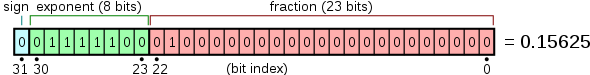
\includegraphics[width=\textwidth]{Notes/Figures/Float_example.png}
\end{figure}
This is the \red{IEEE 754} standard: everybody must agree how to parse the bits, otherwise it is a mess!\\


\red{Exercise}: you have a simple program that given a floating point input gives you the bit representation as in the figure above, plus the decomposition in powers of $2$. \\
What are your observations? How is the number formatted? 


\end{frame}


\subsection{All good, but then what?}
\begin{frame}{How does we instruct the computer}
\begin{columns}
\begin{column}{0.45\textwidth}
\begin{figure}
    \centering
    \includestandalone[width=\textwidth]{Notes/Figures/instruction_diagram}
\end{figure}
\end{column}
\begin{column}{0.55\textwidth}
How does it work (\red{in a very approximate way})?\\
\green{Level 0}: BIOS/UEFI = basic software built-in in the motherboard, manages the very low level hardware\\
\green{Level 1}: OS = manages all the software, it is loaded by the BIOS/UEFI by reading instructions off a particular region of the memory\\
\green{Level 2}: programs = the OS manages your programs, the memory for each of them, where they store information etc.
\end{column}
\end{columns}
\end{frame}

\begin{frame}[fragile]{How does we instruct the computer}
On a 64 bit machine each instruction can be up to 15 \red{bytes} long(!). The 64 bit refers to the maximum size of each \red{register} in the cpu.\\
Each instruction is \red{literally} a sequence of $0,1$ that triggers some electronics to do `stuff', like adding two numbers, moving memory, jump to different addresses etc.\\
It is not manageable to write instructions in binary (or hex) format: human-readable machine code $\sim \text{assembly 
\includegraphics[width=0.04\textwidth]{Notes/Figures/assm.png}}$
\begin{columns}
\begin{column}{0.55\textwidth}
\raggedleft
\small
\begin{lstlisting}[language={[x86masm]Assembler}]
push rbp
mov  rbp, rsp
mov  DWORD PTR [rbp-4], 1
mov  DWORD PTR [rbp-8], 2
mov  edx, DWORD PTR [rbp-4]
mov  eax, DWORD PTR [rbp-8]
add  eax, edx
mov  DWORD PTR [rbp-12], eax
mov  eax, 0
pop  rbp
ret
\end{lstlisting}
\end{column}
\begin{column}{0.45\textwidth}
More readable than a buch of $1$ and $0$, but still a long way from its C counterpart:
\begin{lstlisting}[language={[x86masm]Assembler}]
int a = 1;
int b = 2;
int c = a + b;
\end{lstlisting}

\end{column}
\end{columns}
\end{frame}

\begin{frame}{Programming languages}
\begin{figure}
    \centering
    \includestandalone[width=0.5\textwidth]{Notes/Figures/programming_languages}
\end{figure}
\end{frame}

\begin{frame}{Examples}
What does it mean to `compile' a language? \\
\[
\text{Human-readable code} \Longrightarrow \text{Machine code}
\]
It is a translation!
\\
{\color{redgray} \textbf{Python}}: interpreted language. What does it mean? It reads the commands, parse them, construct \red{on the fly} the logical tree and execute them via previously compiled functions.\\
{\color{bluegray} \textbf{Lua}}: JIT (just-in-time compiled) language. It reads pieces of code, \red{compile them on-the-fly} and execute the resulting binary.\\{\color{greengray} \textbf{C/C++}}: compiled languages. There is a dedicated piece of software (the compiler) that translates the code to machine instructions. This is done \red{separately} from the running of the program itself.
\end{frame}

\begin{frame}
Programming languages (or syntaxes) come in all shape and form!\\
Not all of them are friendly: in the beginning select the language that feels most natural to you, then you should keep in mind to use \red{the right tool for the job}.\\
For instance, did you know that you can programm a roller coaster in Excel? \href{https://www.youtube.com/watch?v=IrVA1BBHFHw}{Link}\\
Or that it does exist a (Turing complete!) programming language with just 8 symbols? It is called \href{https://en.wikipedia.org/wiki/Brainfuck}{Brainfuck} (guess why...) and to print the string `Hello World!' the code is 
\[\begin{split}
& ++++++++[>++++[>++>+++>+++\\
& >+<<<<-]>+>+>->>+[<]<-]\\
& >>.>---.+++++++..+++.>>.<-.\\
& <.+++.------.--------.>>+.>++.
\end{split}\]
Crazy, ain't it?
\end{frame}

\begin{frame}
Your turn now, let us play a bit!
\end{frame}

\section{Neural Networks, the basics}


\bibliography{Notes/biblio}
\end{document}